\section{Inleiding}
Binnen software engineering is UML een veelgebruikt gereedschap om het domein waarin de software die ontworpen wordt alsook de structuur van de software zelf grafisch weer te geven. Het is voor de ontwerper interessant om uit een tekstuele beschrijving van wat de voorgestelde software moet kunnen de relevante concepten en procedures te halen, die neer te zetten in een diagram en door middel van de verscheidene symbolen aangeboden door UML uit te drukken hoe die concepten en procedures met elkaar interageren. Op deze manier kan een team snel duidelijkheid scheppen in welke doelen ze precies moeten bereiken.

Het is echter makkelijk om het overzicht te verliezen als de gebruikte diagrammen omvangrijk worden. Dit kan een probleem zijn omdat fouten die worden gemaakt in de ontwerpfase en pas laat in het productieproces ontdekt worden kostbaar zijn om recht te zetten. Het komt ook voor dat een ontwerper per vergissing overbodige informatie toevoegt aan een diagram en dat daardoor het diagram minder duidelijk wordt.

In deze masterproef worden in het bijzonder UML-klassediagrammen beschouwd. Een klassediagram beschrijft welke concepten (in deze tekst verder \textit{klasses} genoemd) er bestaan binnen de software. Elk van die klasses kan attributen en operaties hebben. Verder geeft een klassediagram ook weer welke klasses in relatie staan tot elkaar. Deze relaties leggen vast aan welke beperkingen alle mogelijke toestanden van de beschreven software moeten voldoen om beschouwd te worden als correct.

Beschouw volgend klassediagram:

\begin{figure}[H]
	\label{fig:cd}
	\centering
	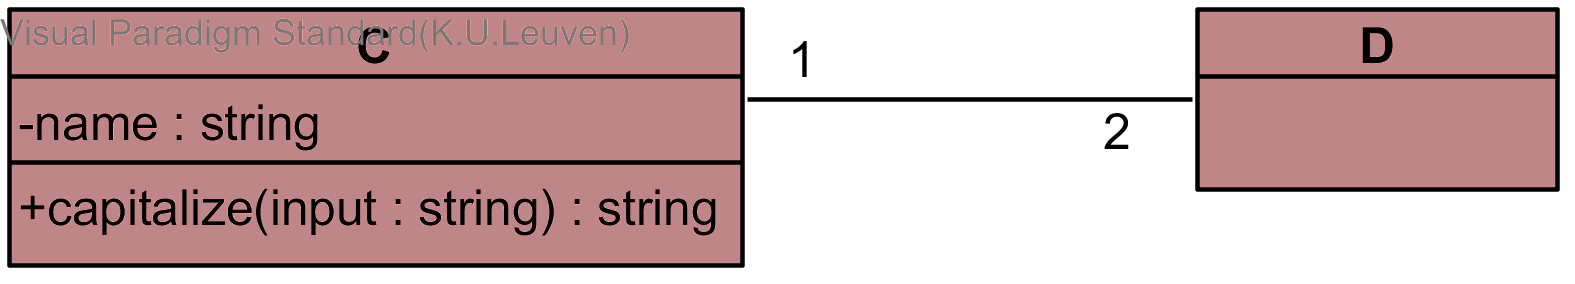
\includegraphics{intro/cd.png}
	\caption{Een voorbeeld van een klassediagram}
\end{figure}

Dit klassediagram drukt uit dat er twee klasses bestaan: \textit{C} en \textit{D}. \textit{C} heeft \'e\'en attribuut, \textit{name}, dat van type \textit{string} is. Het heeft ook \'e\'en operatie \textit{capitalize} dat \textit{input}, van type \textit{string}, als parameter heeft. \textit{capitalize} geeft een resultaat terug dat ook van type \textit{string} is. Voorts drukt de lijn tussen \textit{C} en \textit{D} uit dat er een relatie bestaat tussen de twee klasses. Beschouw klasse C. Als we vanuit die klasse de lijn volgen, zien we dat er aan het ander uiteinde staat dat elke \textit{C}-object in relatie moet staan tot exact twee \textit{D}-objecten. Zo ook zien we dat, als we vertrekken vanuit \textit{D}, elk \textit{D}-object in relatie moet staan tot exact \'e\'en \textit{C}-object.

Met het voorgaande in het achterhoofd beschouwen we in deze masterproef twee categorie\"en van gebreken in een klassediagram:

\begin{itemize}
	\item \textbf{Inconsistenties:} Het klassediagram is zo opgebouwd dat geen enkele mogelijke toestand van de software kan beantwoorden aan de voorwaarden die worden opgelegd. Dit betekent dat het stuk van de software dat wordt beschreven in het diagram onmogelijk kan werken.
	\item \textbf{Kwaliteitsgebreken:} Deze gebreken hebben een negatieve impact op de kwaliteit van het softwareontwerp. Zo kunnen ze bijvoorbeeld onduidelijkheden in het ontwerp introduceren of het onderhoud van de software \'e\'enmaal ingezet in productie bemoeilijken.
\end{itemize}

Deze masterproef heeft tot doel om automatisch op een gestructureerde manier uit te drukken welke informatie een UML-klassediagram juist bevat. Die informatie willen we op zijn beurt terug gebruiken om inconsistenties en kwaliteitsgebreken te detecteren. Concreter willen we predikatenlogica gebruiken om de informatie neer te schrijven en om aan detectie van gebreken te doen. De volgende hoofdstukken beschrijven hoe we dit exact willen bereiken. \todo{relevante structuur van document beschrijven}